% Documento de Teste com Imagem
\documentclass[12pt,a4paper]{article}

% Pacotes essenciais
\usepackage[utf8]{inputenc}
\usepackage[portuguese]{babel}
\usepackage[T1]{fontenc}
\usepackage{graphicx}

% Informações do documento
\title{Teste com Imagem}
\author{DocCollab}
\date{\today}

\begin{document}

\maketitle

\section{Introdução}

Este é um documento de teste com uma imagem.

\section{Imagem}

A Figura \ref{fig:frog} mostra um sapo.

\begin{figure}[h]
  \centering
  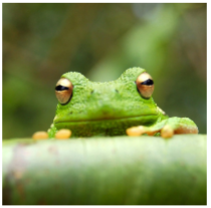
\includegraphics[width=0.5\textwidth]{imagens/frog.png}
  \caption{Um sapo verde}
  \label{fig:frog}
\end{figure}

Como podemos ver na Figura \ref{fig:frog}, a imagem foi incluída com sucesso.

\section{Conclusão}

O sistema está funcionando corretamente!

\end{document}


